\documentclass[a4paper,12pt]{article} 


\usepackage[T2A]{fontenc}			% кодировка
\usepackage[utf8]{inputenc}			% кодировка исходного текста
\usepackage[english,russian]{babel}	% локализация и переносы


% Математика
\usepackage{amsmath,amsfonts,amssymb,amsthm,mathtools} 

\usepackage{gensymb}	
\usepackage{wasysym}

% Картинки
\usepackage{graphicx}
\graphicspath{{images/}}

%Заговолок
\usepackage[left=2cm,right=2cm,
    top=2cm,bottom=2cm,bindingoffset=0cm]{geometry}

\usepackage{titling}


\author{Петров Артём Антонович, группа 721}
\title{"Лабораторная работа № x.x.x "name"}
\date{\today}

\begin{document} % начало документа

\begin{minipage}[t][8cm]{\textwidth}
\maketitle
\end{minipage}


\textbf{Цель работы:} 
\bigskip

\textbf{Оборудование:} 
\bigskip

\textbf{Теория}
\bigskip


\bigskip

\textbf{Установка:}
\medskip


\begin{figure}[ht]
\centering
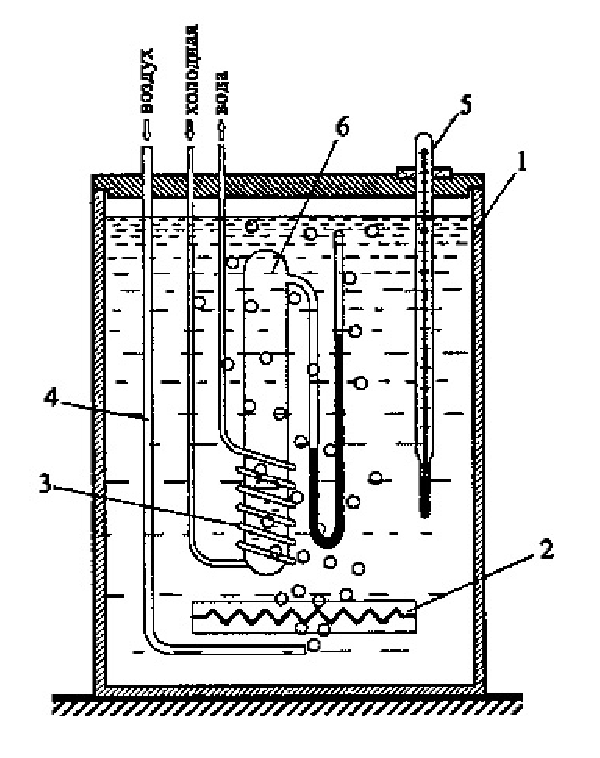
\includegraphics[width=80mm]{schema.eps}
\caption{Схема установки: }\label{schema}
\end{figure}

\bigskip

\textbf{Ход работы:}
\bigskip


\bigskip

\textbf{Записи из журнала:}
\bigskip


\bigskip

\textbf{Итог:}
\bigskip
 
\end{document} % конец документа